\section{Ergebnisse aus Simulatorrecherche}\label{chap:results_sim}

\sh{Allgemeine Informationen}
Abbildung~\ref{fig:1-anzahl-jahr} verdeutlicht, dass der Großteil der untersuchten Simulatoren zu Beginn der 2000er-Jahre veröffentlicht wurde. Zwischen 2000 und 2020 lassen sich insgesamt 37 Veröffentlichungen identifizieren, was einem Anteil von 74~\% entspricht. Darüber hinaus konnte bei sieben Simulatoren kein Veröffentlichungsdatum ermittelt werden.

Hinsichtlich des Wartungsstands der bereits veröffentlichten Simulatoren zeigt Abbildung~\ref{fig:2-veroeffentlichungen}, dass dieser im Zeitverlauf zunimmt. Etwa 71~\% der Simulatoren wurden in den vergangenen fünf Jahren aktualisiert und können somit als \enquote{aktuell} eingestuft werden.

\begin{figure}[!htbp]
    \centering
    % --- linke Seite: Grafik ---
    \begin{subfigure}[b]{0.48\textwidth}
        \centering
        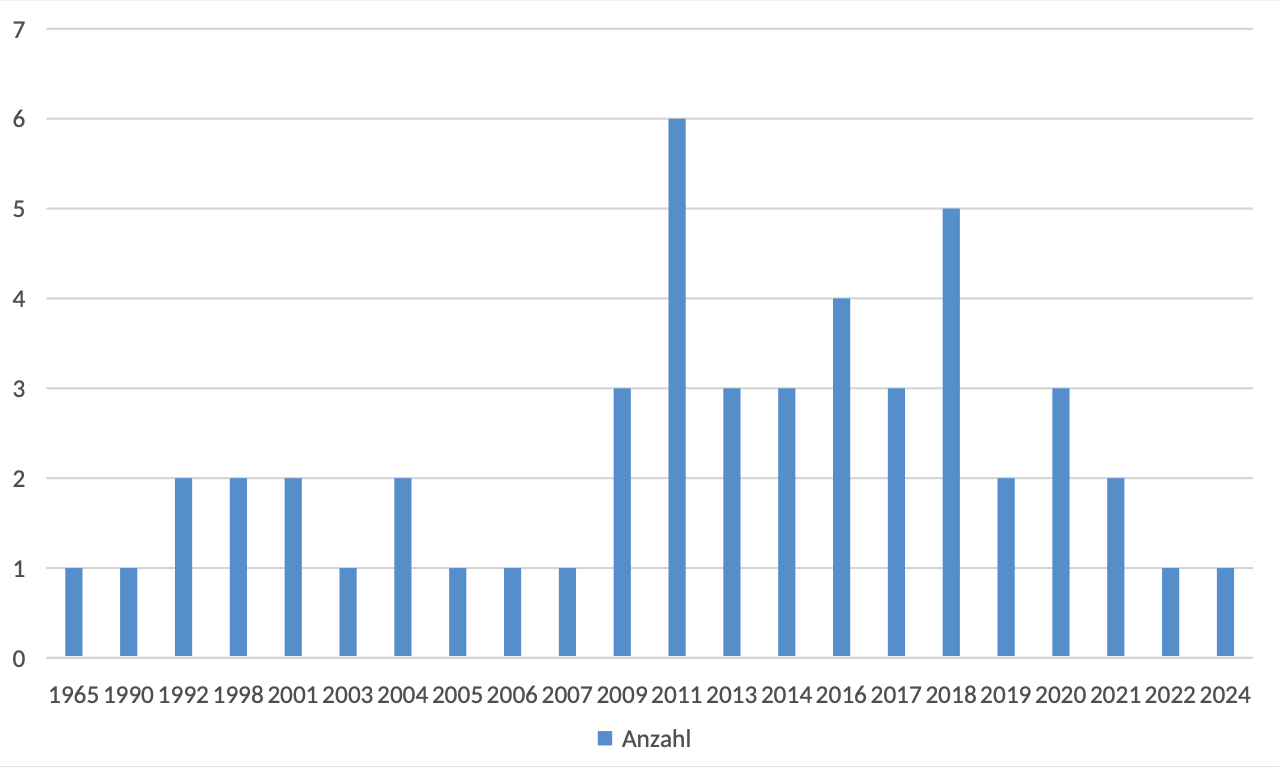
\includegraphics[width=0.90\textwidth]{graphics_sim/1-anzahl-jahr.png}
        \caption{Jährliche Übersicht der Veröffentlichungen}
        \label{fig:1-anzahl-jahr}
    \end{subfigure}
    \hfill
    % 
    % --- rechte Seite: Grafik ---
    \begin{subfigure}[b]{0.48\textwidth}
        \centering
        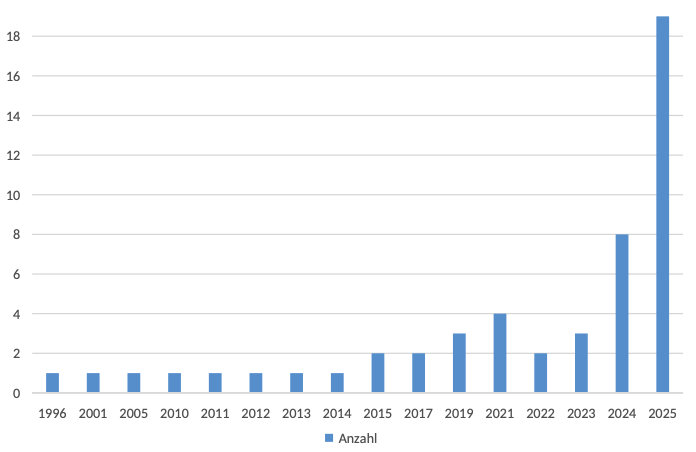
\includegraphics[width=0.90\textwidth]{graphics_sim/2-veroeffentlichung.png}
        \caption{Jährliche Übersicht des Wartungsstands}
        \label{fig:2-veroeffentlichungen}
    \end{subfigure}
    %
    \caption{Analysen zum Jahr der Veröffentlichung und zum Wartungsstand}
    \label{fig:veroeffentlichung_wartungsstand}
\end{figure}

\sh{Chronologische Entwicklung}
Die thematische Verteilung der Simulatoren ist Abbildung~\ref{fig:7-thema} zu entnehmen. Etwa 40~\% der Simulatoren befassen sich mit dem Themenbereich \enquote{Prozessoren und Architekturen}, gefolgt von 18~\% hardwarebezogenen und 14~\% grundlagenvermittelnden Simulatoren. Die übrigen Anwendungen verteilen sich auf die Themenbereiche \enquote{Speicher und Performance}, \enquote{Programmierung}, \enquote{Systeme und Anwendungen}, \enquote{GPU} sowie \enquote{Monitoring}.

Die Zuordnung der Veröffentlichungsjahre zu den Zeiträumen \enquote{vor 2000}, \enquote{2000 -- 2010}, \enquote{2010 -- 2020} und \enquote{nach 2020} ist in Abbildung~\ref{fig:8-thema-jahr} dargestellt. Hier wird deutlich, dass die Mehrheit der Simulatoren zum Themenbereich \enquote{Prozessoren und Architekturen} im Zeitraum 2010 bis 2020 veröffentlicht wurde.

Wie bereits in der Literaturrecherche sind auch in der Simulatorrecherche die Themenbereiche \enquote{Prozessoren und Architekturen} sowie \enquote{Hardware und Logik} am stärksten vertreten. Unter den 49~\% der untersuchten Simulatoren treten insbesondere die Subthemen \enquote{RISC} und \enquote{Digitale Logik} am häufigsten auf. Damit lassen sich vergleichbare Entwicklungen in beiden Analysen feststellen.

Die verbleibenden Themenbereiche liefern in Bezug auf die zeitliche Entwicklung anhand des Veröffentlichungsjahres keine weiterführenden Erkenntnisse. Auch aus dem Wartungsstand der untersuchten Simulatoren lassen sich keine eindeutigen Trends ableiten. Wie Abbildung~\ref{fig:2-veroeffentlichungen} zeigt, befinden sich die meisten Simulatoren im Wesentlichen auf einem aktuellen Entwicklungsstand. Das gewichtete arithmetische Mittel pro Themenbereich liegt nicht vor dem Jahr 2018.


\begin{figure}[!htbp]
    \centering
    % --- linke Seite: Grafik ---
    \begin{subfigure}[b]{0.48\textwidth}
        \centering
        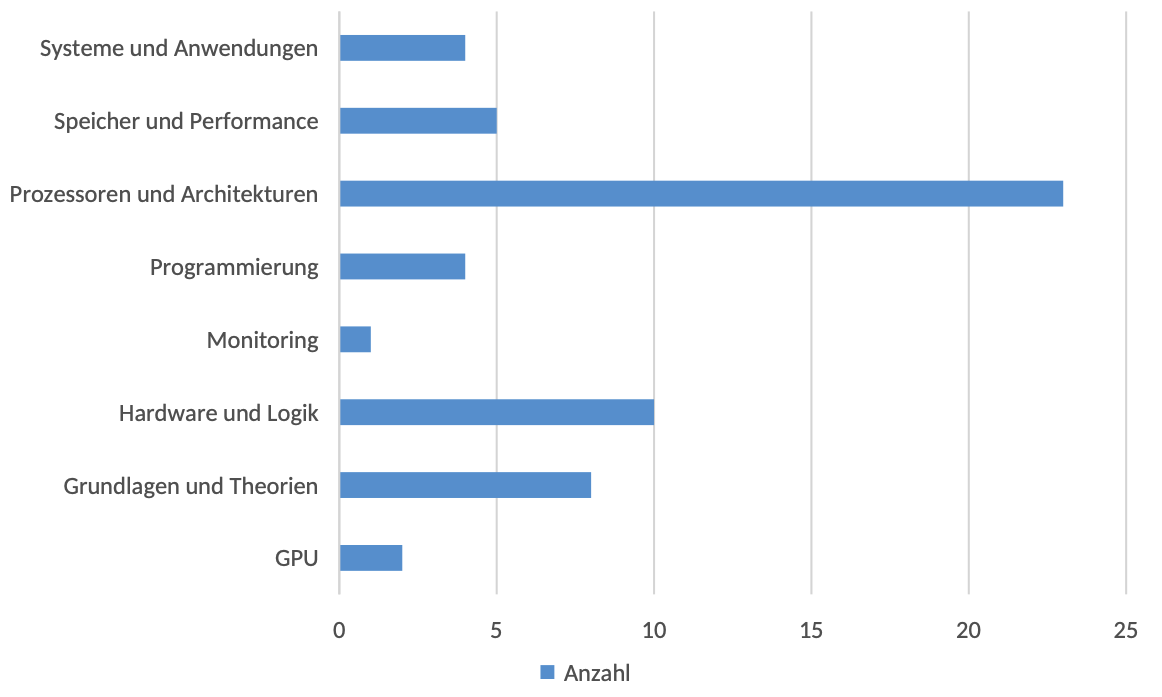
\includegraphics[width=0.90\textwidth]{graphics_sim/7-thema.png}
        \caption{Übersicht der Themenverteilung}
        \label{fig:7-thema}
    \end{subfigure}
    \hfill
    % 
    % --- rechte Seite: Grafik ---
    \begin{subfigure}[b]{0.48\textwidth}
        \centering
        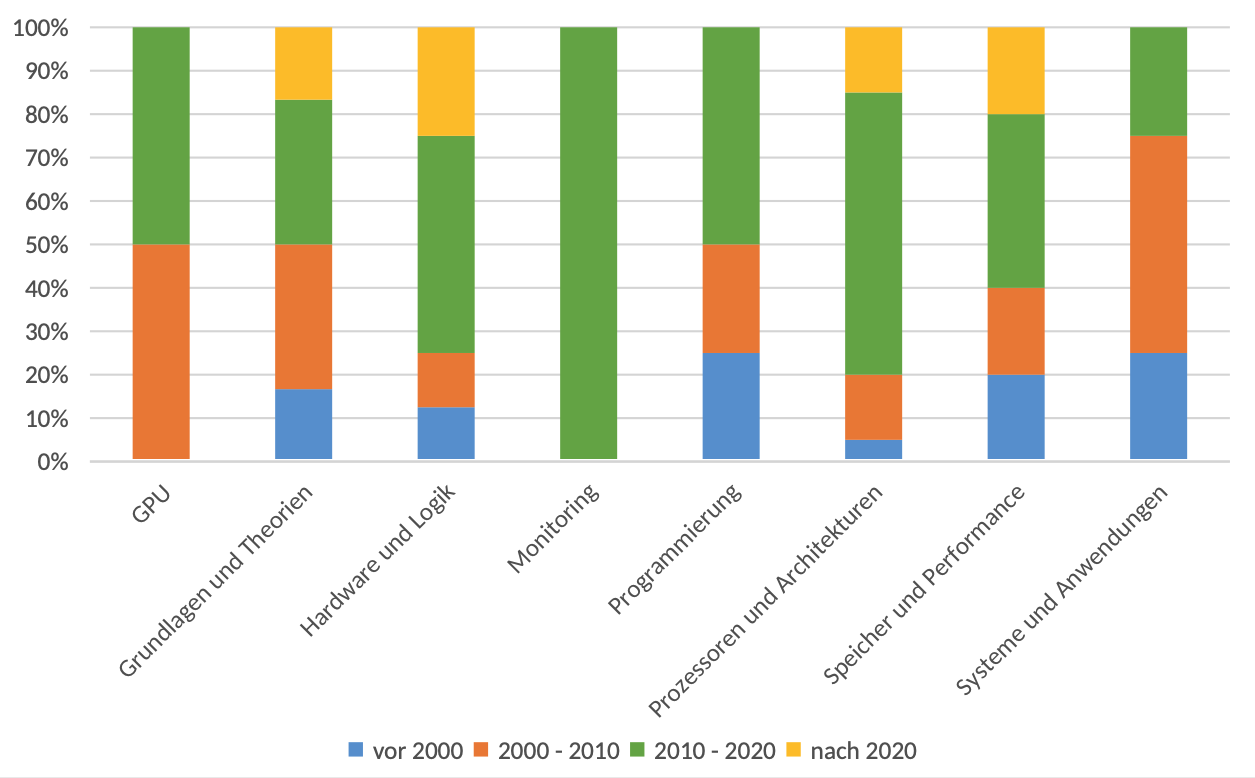
\includegraphics[width=0.90\textwidth]{graphics_sim/8-thema-jahr.png}
        \caption{Jährliche Übersicht der Themenverteilung}
        \label{fig:8-thema-jahr}
    \end{subfigure}
    %
    \caption{Analysen zur Themenverteilung}
    \label{fig:themen-gesamt}
\end{figure}

\sh{Gamification}
Hinsichtlich des Kriteriums Gamification ist festzuhalten, dass die in Tabelle~\ref{tab:simulatoren} aufgeführten Simulatoren keine spielerischen Elemente enthalten und dieses Kriterium daher keine Aussagekraft hier bietet.

\sh{Abstraktionslevel}
Im Rahmen der Simulatorrecherche wird auch das Abstraktionsniveau erfasst (vgl. Abbildung~\ref{fig:5-abstraktion}). Der überwiegende Teil (ca. 72~\%) der Simulatoren ist dabei als \enquote{didaktisch reduziert} zu klassifizieren. Diese Simulatoren verteilen sich gemäß Abbildung~\ref{fig:6-abstraktion-thema} im Wesentlichen auf die Themenbereiche \enquote{Prozessoren und Architekturen} sowie \enquote{Hardware und Logik}.

\begin{figure}[!htbp]
    \centering
    % --- linke Seite: Grafik ---
    \begin{subfigure}[b]{0.48\textwidth}
        \centering
        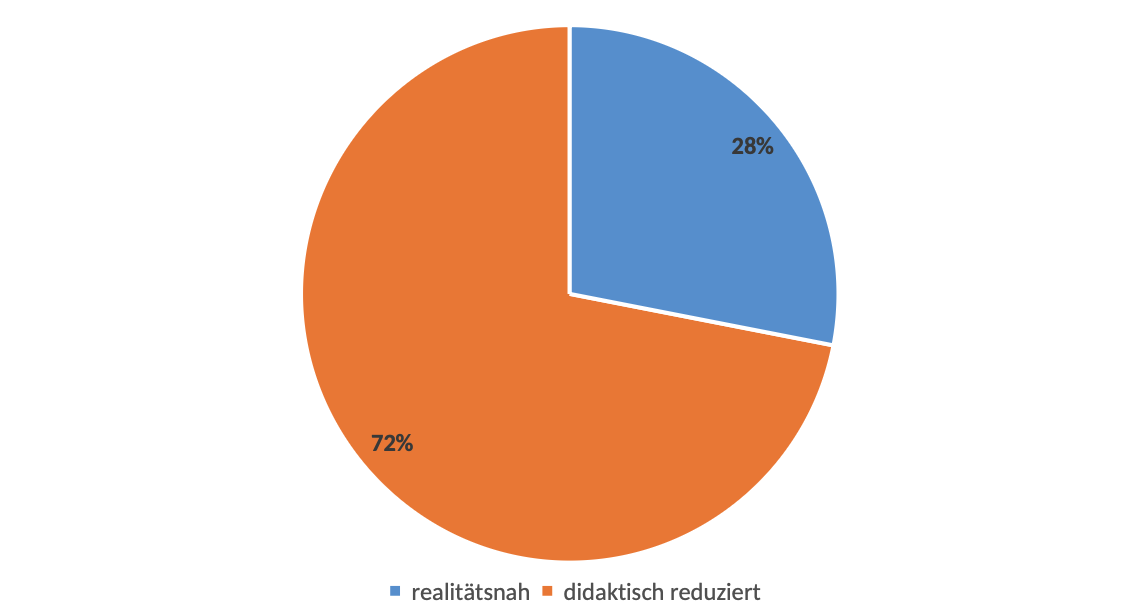
\includegraphics[width=0.90\textwidth]{graphics_sim/5-abstraktion.png}
        \caption{Übersicht der Abstraktionslevel}
        \label{fig:5-abstraktion}
    \end{subfigure}
    \hfill
    % 
    % --- rechte Seite: Grafik ---
    \begin{subfigure}[b]{0.48\textwidth}
        \centering
        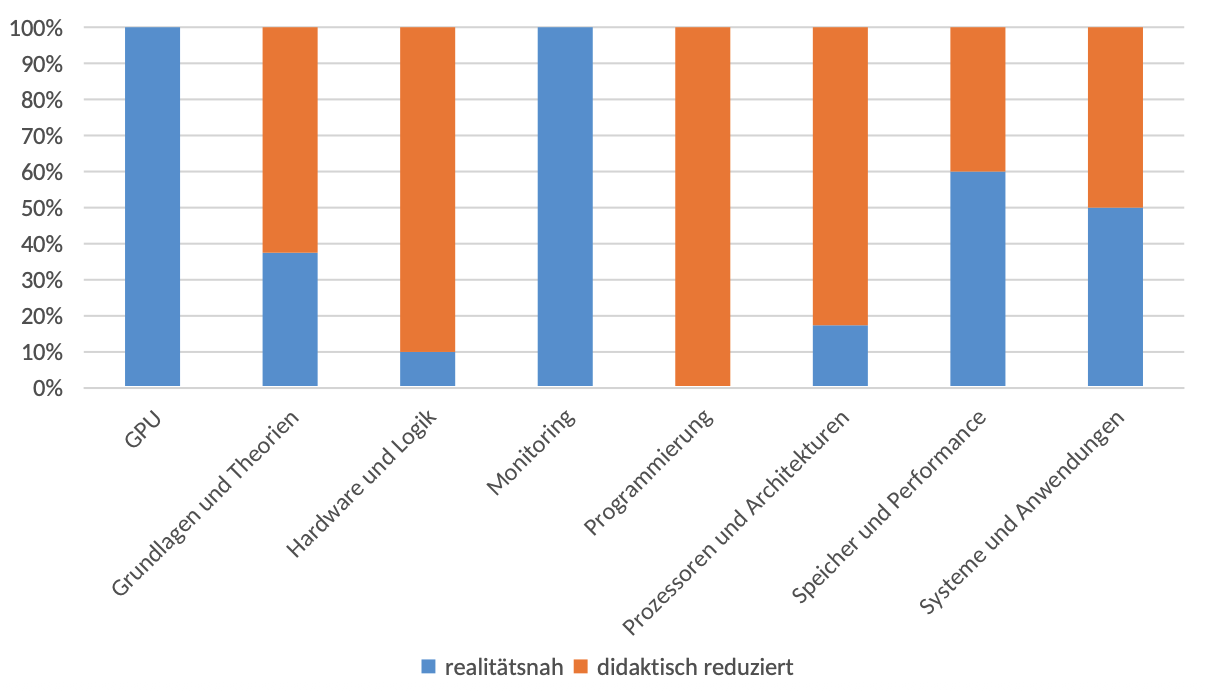
\includegraphics[width=0.90\textwidth]{graphics_sim/6-abstraktion-thema.png}
        \caption{Übersicht der Abstraktionslevel pro Thema}
        \label{fig:6-abstraktion-thema}
    \end{subfigure}
    %
    \caption{Analysen zum Abstraktionslevel}
    \label{fig:abstraktion-gesamt}
\end{figure}

Neben dem Abstraktionsniveau wird auch die Zielgruppe der jeweiligen Simulatoren betrachtet. Dabei erfolgt eine Unterscheidung zwischen den Kategorien \enquote{Schule}, \enquote{Hochschule} sowie \enquote{Forschung, Beruf}. Da eine Anwendung potenziell für mehrere Zielgruppen relevant sein kann und somit mehreren Kategorien zugeordnet wird, wird auf eine grafische Darstellung verzichtet. Tabelle~\ref{tab:institutionen} bietet stattdessen eine Übersicht über die Verteilung der Simulatoren auf die jeweiligen Institutionstypen.

\begin{table}[h]
	\centering
	\caption{Verteilung der Institutionstypen}
	\label{tab:institutionen}
	\begin{tabular}{l r}
		\toprule
		\textbf{Institution(en)} & \textbf{Anzahl} \\
		\midrule
		Schule                        & 7  \\
		Schule, Hochschule            & 2  \\
		Hochschule                    & 31 \\
		Hochschule, Forschung, Beruf  & 14 \\
		Forschung, Beruf              & 3  \\
		\bottomrule
	\end{tabular}
\end{table}

Analog zur Literaturrecherche sind auch innerhalb der untersuchten Simulatoren der überwiegende Teil didaktisch reduziert. In den Themenbereichen \enquote{GPU} und \enquote{Monitoring} besteht das Die Recherche hingegen ausschließlich aus realitätsnahen Simulatoren.

Die Erkenntnis, dass Simulatoren für die Hochschulbildung überwiegend didaktisch reduziert sein sollten, wird durch die Grundgesamtheit der veröffentlichten Simulatoren bestätigt. Die 72~\% didaktisch reduzierten Simulatoren richten sich vollständig an die Zielgruppen \enquote{Schule} und \enquote{Hochschule}.

Da in dieser Arbeit überwiegend didaktische reduzierte Simulatoren vorgestellt werden, ist das Kriterium \enquote{Vorwissen} von besonderem Interesse. Etwa 77~\% der Simulatoren setzen Grundkenntnisse in den jeweiligen Themengebieten voraus (vgl. Abbildung~\ref{fig:10-vorwissen}). Rund 5~\% erfordern fortgeschrittene Kenntnisse, während lediglich 18~\% ohne Vorkenntnisse genutzt werden können. Die Verteilung nach Themengebieten in Verbindung mit dem erforderlichen Vorwissen ist in Abbildung~\ref{fig:11-vorwissen-thema} dargestellt.

\begin{figure}[!htbp]
    \centering
    % --- linke Seite: Grafik ---
    \begin{subfigure}[b]{0.48\textwidth}
        \centering
        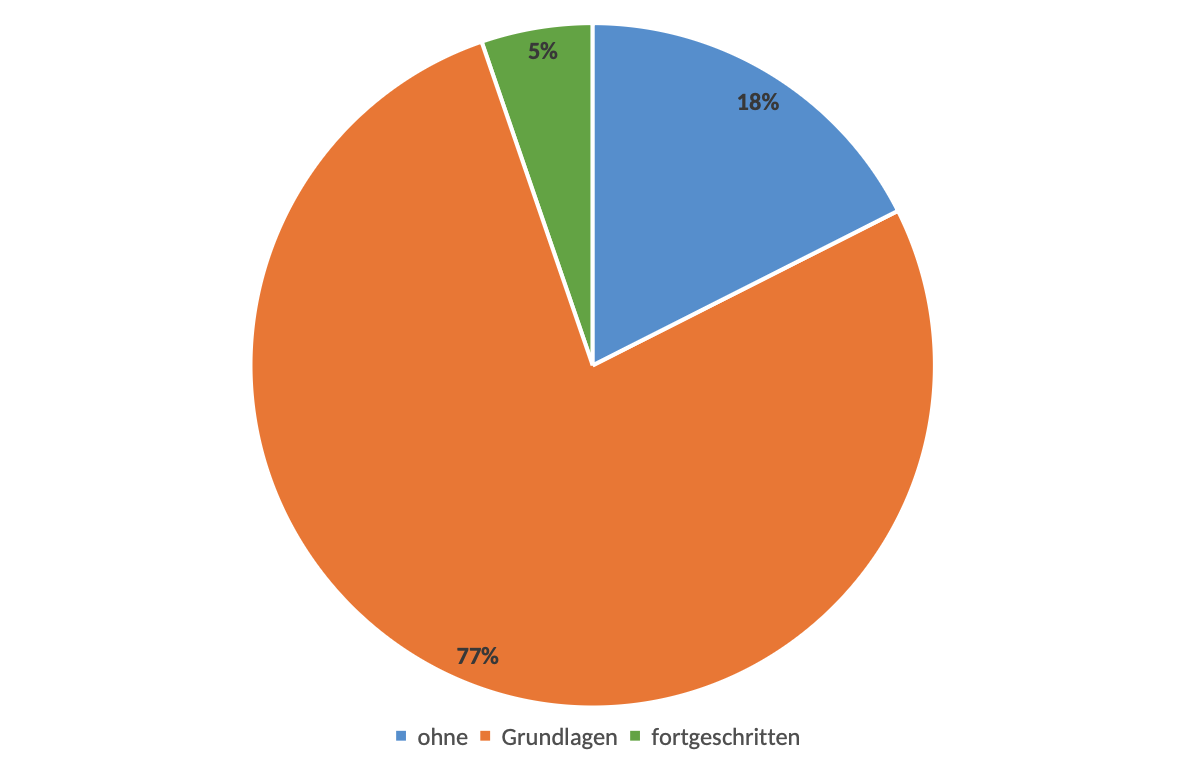
\includegraphics[width=0.90\textwidth]{graphics_sim/10-vorwissen.png}
        \caption{Verteilung Vorwissen}
        \label{fig:10-vorwissen}
    \end{subfigure}
    \hfill
    % 
    % --- rechte Seite: Grafik ---
    \begin{subfigure}[b]{0.48\textwidth}
        \centering
        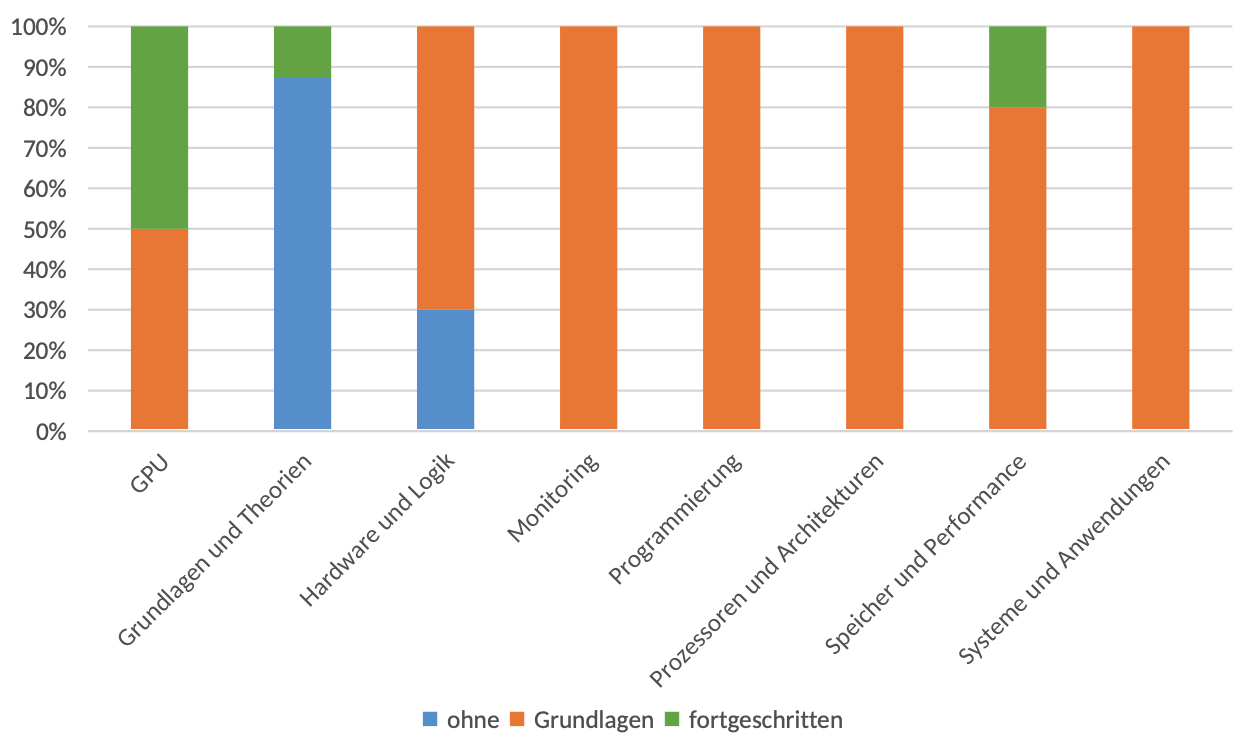
\includegraphics[width=0.90\textwidth]{graphics_sim/11-vorwissen-thema.png}
        \caption{Verteilung Vorwissen auf Themen}
        \label{fig:11-vorwissen-thema}
    \end{subfigure}
    %
    \caption{Analysen Vorwissen}
    \label{fig:vorwissen-gesamt}
\end{figure}

Im Kontext schulischer und hochschulbezogener didaktischer Simulatoren ist das Vorwissen auch mit Blick auf lernpsychologische Theorien (vgl. Kapitel~\ref{chap:3-1-psychology}) von besonderem Interesse:

\begin{itemize}
    \item \textit{\ac{CTML}}: Als Faktor für das \textit{Active Processing} kann Vorwissen unterstützen, neue Informationen sinnvoll zu verarbeiten und an bestehende mentale Modelle anzuknüpfen.
    \item \textit{Exploratives Lernen}: Vorwissen ermöglicht Lernenden, Hypothesen zu entwickeln, Simulationen gezielt durchzuführen und daraus tragfähige Schlussfolgerungen zu ziehen.
    \item \textit{Erfahrungsbasiertes Lernen}: Hier fungiert Vorwissen als Ausgangspunkt, auf dem neue Erfahrungen aufbauen. Es erleichtert die Phase der \textit{reflektierenden Beobachtung}, da neue Eindrücke mit vorhandenen Konzepten verglichen und kritisch eingeordnet werden können.
    \item \textit{Konnektivismus}: Vorwissen stellt ein Geflecht aus Wissensknoten dar. Dieses Netzwerk ermöglicht es, neue Informationen in bestehende Strukturen einzubetten und durch Verknüpfungen mit externen Ressourcen zu erweitern.
\end{itemize}

\sh{Zugriff}
 Die Zugriffsart wird in Abbildung~\ref{fig:3-zugriff} dargestellt. Den größten Anteil bilden offline nutzbare Simulatoren (53~\%). Etwa 11~\% der Simulatoren sind sowohl online als auch offline verfügbar, während 37~\% ausschließlich online zugänglich sind.

Abbildung~\ref{fig:4-zugriff-jahr} verdeutlicht, wie sich die Zugriffsarten im Zeitverlauf entwickelt haben.

\begin{figure}[!htbp]
    \centering
    % --- linke Seite: Grafik ---
    \begin{subfigure}[b]{0.48\textwidth}
        \centering
        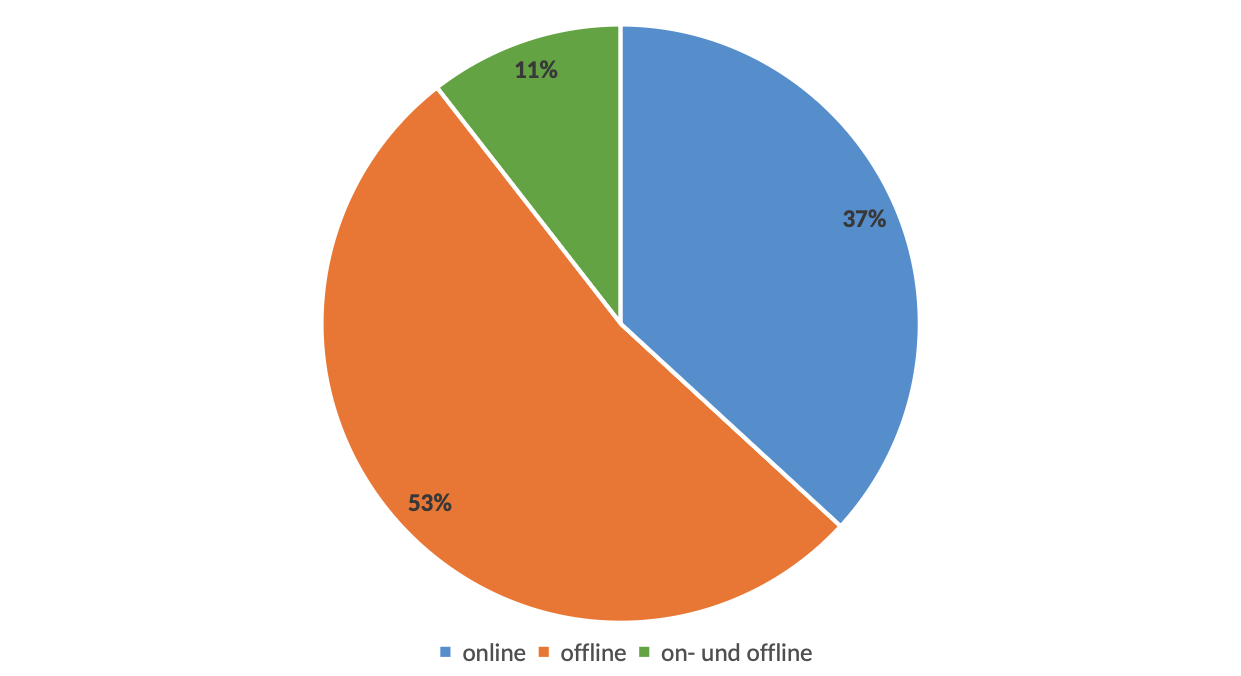
\includegraphics[width=0.90\textwidth]{graphics_sim/3-zugriff.png}
        \caption{Übersicht der Zugriffsarten}
        \label{fig:3-zugriff}
    \end{subfigure}
    \hfill
    % 
    % --- rechte Seite: Grafik ---
    \begin{subfigure}[b]{0.48\textwidth}
        \centering
        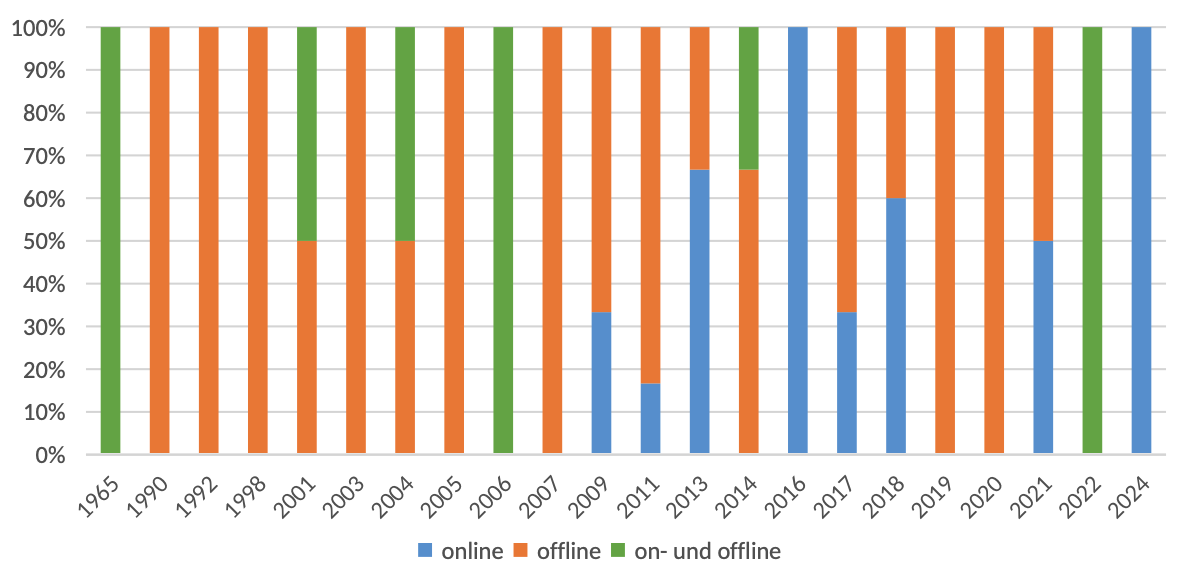
\includegraphics[width=0.90\textwidth]{graphics_sim/4-zugriff-jahr.png}
        \caption{Jährliche Übersicht der Zugriffsarten}
        \label{fig:4-zugriff-jahr}
    \end{subfigure}
    %
    \caption{Analysen zur Zugriffsart}
    \label{fig:zugriff-gesamt}
\end{figure}

Bezogen auf das Kriterium \ac{OS} wird keine Abbildung dargestellt, da einzelne Simulatoren mehreren Betriebssystemen zugeordnet werden können. Stattdessen zeigt Tabelle~\ref{tab:os} die Verteilung der Simulatoren auf die jeweiligen Betriebssysteme. Auffällig ist, dass der größte Anteil als \enquote{unabhängig} klassifiziert ist. Diese Simulatoren sind online verfügbar und damit nicht an ein spezifisches Betriebssystem gebunden. In der Kategorie \enquote{unabhängig} wurden rund 19~\% der Simulatoren im Zeitraum 2010 bis 2020 veröffentlicht, weitere 14~\% in den Jahren 2020 bis 2025.

\begin{table}[h]
	\centering
	\caption{Verteilung der unterstützten Betriebssysteme}
	\label{tab:os}
	\begin{tabular}{l r}
		\toprule
		\textbf{Betriebssystem(e)} & \textbf{Anzahl} \\
		\midrule
		Linux                     & 4  \\
		Linux, Windows            & 1  \\
		Linux, Windows, macOS     & 11 \\
		Windows                   & 1  \\
		Windows, \ac{VM}          & 1  \\
		\ac{VM}                   & 2  \\
		unabhängig                & 37 \\
		\bottomrule
	\end{tabular}
\end{table}

Die Verteilung von online- und offline-nutzbaren Simulatoren ist in dieser Recherche nahezu ausgeglichen (vgl. Abbildung~\ref{fig:3-zugriff}). Aus Abbildung~\ref{fig:4-zugriff-jahr} lassen sich keine eindeutigen zeitlichen Trends ableiten. Der in Kapitel~\ref{3-2-development-sim} beschriebene Effekt des \textit{M-Learning} kann daher nicht bestätigt werden.

Tabelle~\ref{tab:os} zeigt, dass etwa 37~\% der offline-nutzbaren Simulatoren die gängigen Betriebssysteme \enquote{Linux}, \enquote{Windows} und \enquote{macOS} unterstützen. Überwiegend handelt es sich jedoch um betriebssystemagnostische Simulatoren. Diese Simulatoren wurden zu 51~\% in dem Zeitraum zwischen 2010 und 2020 veröffentlicht. Der Trend flacht in den darauffolgenden Jahren ab.

\sh{Preis}
Der überwiegende Teil der Simulatoren ist kostenfrei verfügbar; lediglich 5~\% sind kostenpflichtig. Eine Übersicht der Verteilung zeigt Abbildung~\ref{fig:9-preis}. Somit wird auch hier der finanzielle Druck auf Lehr- und Lernende reduziert.

\begin{figure}[!htbp]
    \centering
    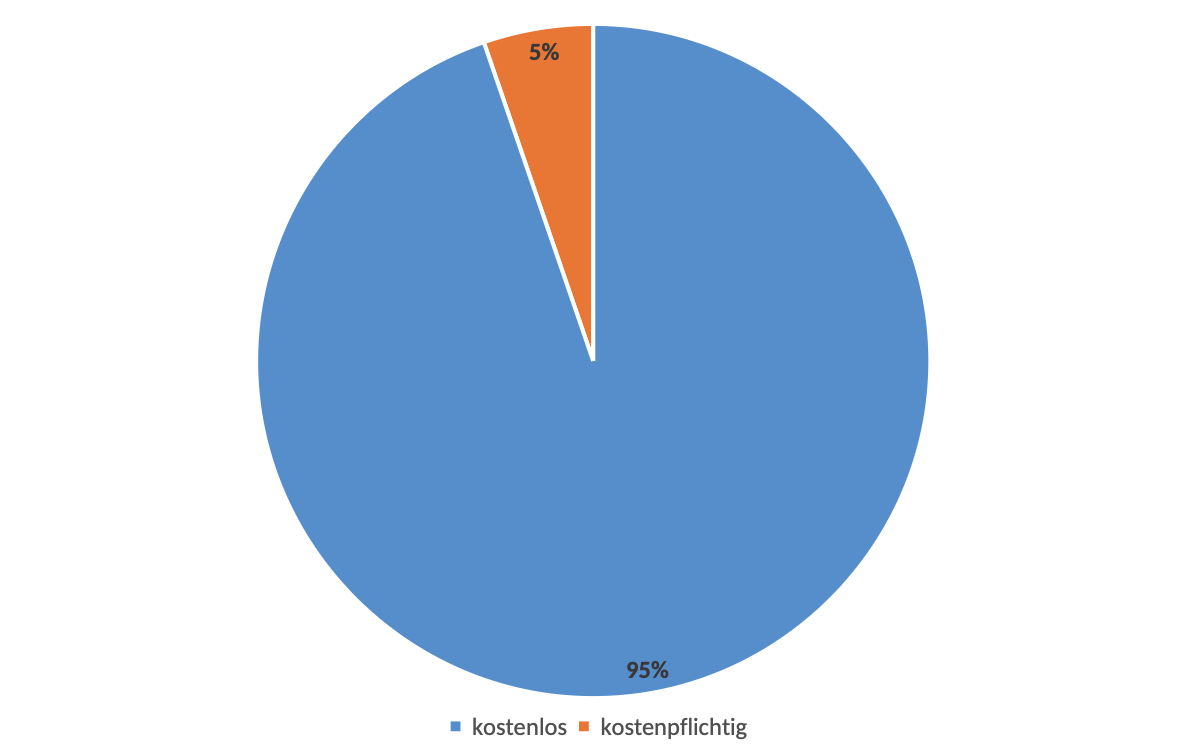
\includegraphics[width=0.90\textwidth]{graphics_sim/9-preis.png}
    \caption{Preisverteilung der veröffentlichten Simulatoren}
    \label{fig:9-preis}
\end{figure}

\sh{Zeit}
Die Abbildungen~\ref{fig:12-zeit} und \ref{fig:13-vorwissen-thema} geben Aufschluss über die Nutzungsdauer der untersuchten Simulatoren. Der überwiegende Teil weist eine kurze Nutzungszeit auf, während lediglich 2~\% eine längere Nutzungsdauer vorsehen. In den Themenbereichen \enquote{Prozessoren und Architekturen} sowie \enquote{Hardware und Logik} finden sich ausschließlich Simulatoren mit kurzer Nutzungszeit.

\begin{figure}[!htbp]
    \centering
    % --- linke Seite: Grafik ---
    \begin{subfigure}[b]{0.48\textwidth}
        \centering
        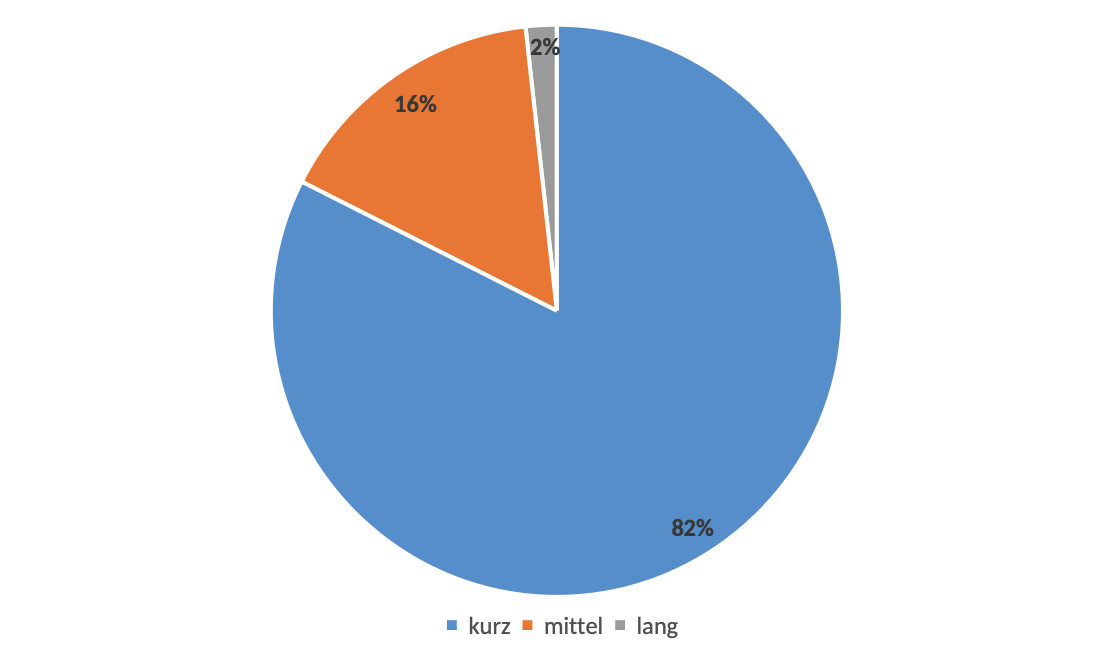
\includegraphics[width=0.90\textwidth]{graphics_sim/12-zeit.png}
        \caption{Verteilung Zeit}
        \label{fig:12-zeit}
    \end{subfigure}
    \hfill
    % 
    % --- rechte Seite: Grafik ---
    \begin{subfigure}[b]{0.48\textwidth}
        \centering
        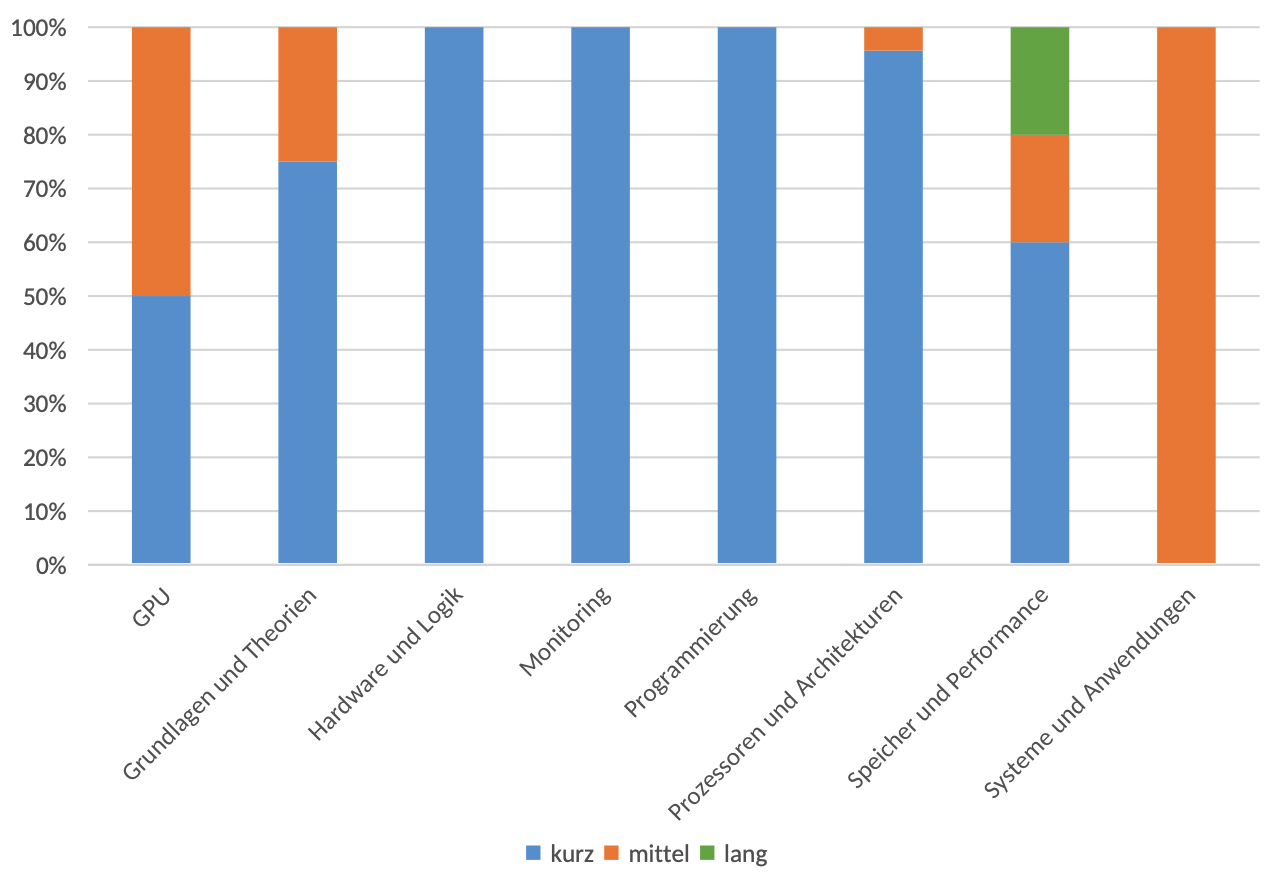
\includegraphics[width=0.90\textwidth]{graphics_sim/13-zeit-thema.png}
        \caption{Verteilung Zeit auf Themen}
        \label{fig:13-vorwissen-thema}
    \end{subfigure}
    %
    \caption{Analysen zur Nutzungsdauer}
    \label{fig:nutzungsdauer-gesamt}
\end{figure}

Die benötigte Bearbeitungszeit eines Simulators lässt in Verbindung zu den lernpsychologischen Theorien aus Kapitel~\ref{chap:3-1-pychology} setzen. Daher ist eine Analyse dieser ebenfalls entscheidend für zukünftige Trends und Best Practices.

Die Analyse des erforderlichen Zeitaufwands (siehe Abbildung~\ref{fig:12-zeit}) zeigt, dass die meisten Simulatoren in kurzer Nutzungsdauer zu Ergebnissen führen. Aus lernpsychologischer Sicht hat dies unterschiedliche Implikationen:

\begin{itemize}
    \item \textit{\ac{CTML}}: Kurze Bearbeitungszeiten können kognitive Überlastung verringern, bergen jedoch die Gefahr, dass für \textit{Active Processing} zu wenig Zeit verbleibt.
    \item \textit{Exploratives Lernen}: Eine geringe Nutzungsdauer schränkt die Möglichkeit ein, eigene Hypothesen ausführlich zu erproben.
    \item \textit{Erfahrungsbasiertes Lernen}: Für die Phase der \textit{reflektierenden Beobachtung} könnte die kurze Dauer unzureichend sein, um Erlebtes nachhaltig zu verarbeiten.
    \item \textit{Konnektivismus}: Die Integration neuer Informationen in bestehende Wissensnetzwerke erfordert mehr Zeit, als viele Simulatoren vorsehen.
\end{itemize}

Aus der Analyse der Nutzungsdauer in Bezug auf die Themen (vgl. Abbildung~\ref{fig:13-vorwissen-thema}) ergeben sich keine zusätzlichen Erkenntnisse. Die höhere Verteilung in den Kategorien \enquote{Hardware und Logik} sowie \enquote{Prozessoren und Architekturen} entspricht der bereits zuvor dargestellten allgemeinen Themenverteilung.

\sh{Dokumentation}
Hinsichtlich der Dokumentation der bereits veröffentlichten Simulatoren zeigt Abbildung~\ref{fig:14-dokumentation}, dass 88~\% der Applikationen über eine ausreichende Begleitdokumentation verfügen. Dieses Ergebnis bestätigt die zuvor dargestellte Relevanz lernpsychologischer Theorien, nach denen eine Dokumentation den Lernprozess wesentlich unterstützt.

\begin{figure}[!htbp]
    \centering
    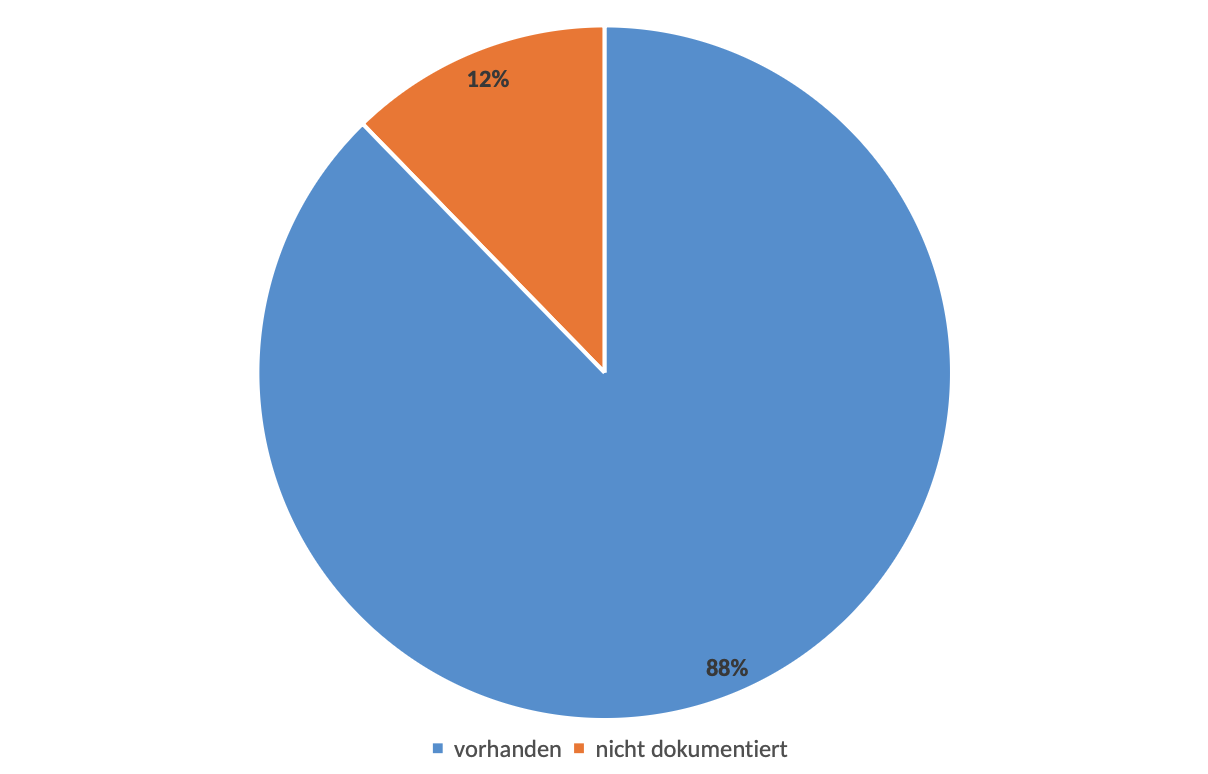
\includegraphics[width=0.90\textwidth]{graphics_sim/14-dokumentation.png}
    \caption{Verteilung der Dokumentation}
    \label{fig:14-dokumentation}
\end{figure}

\sh{Bekanntheit}
Als abschließendes Kriterium wird die Bekanntheit der Simulatoren betrachtet. Insgesamt werden 78~\% der Simulatoren als mittel oder hoch bekannt eingestuft (vgl. Abbildung~\ref{fig:15-bekanntheit}). Eine Übersicht darüber, welche Themenbereiche vergleichsweise geringere Bekanntheit aufweisen, bietet Abbildung~\ref{fig:16-bekanntheit-thema}.

\begin{figure}[!htbp]
    \centering
    % --- linke Seite: Grafik ---
    \begin{subfigure}[b]{0.48\textwidth}
        \centering
        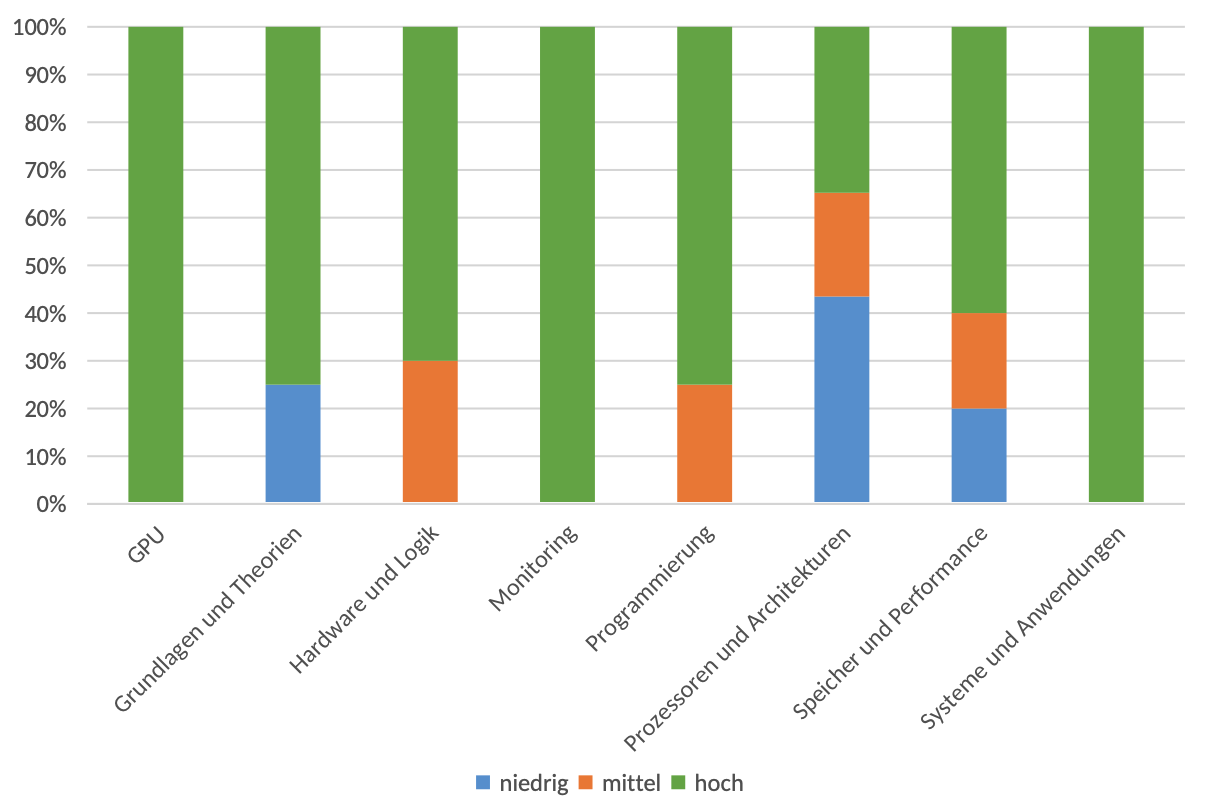
\includegraphics[width=0.90\textwidth]{graphics_sim/15-bekanntheit.png}
        \caption{Verteilung Bekanntheit}
        \label{fig:15-bekanntheit}
    \end{subfigure}
    \hfill
    % 
    % --- rechte Seite: Grafik ---
    \begin{subfigure}[b]{0.48\textwidth}
        \centering
        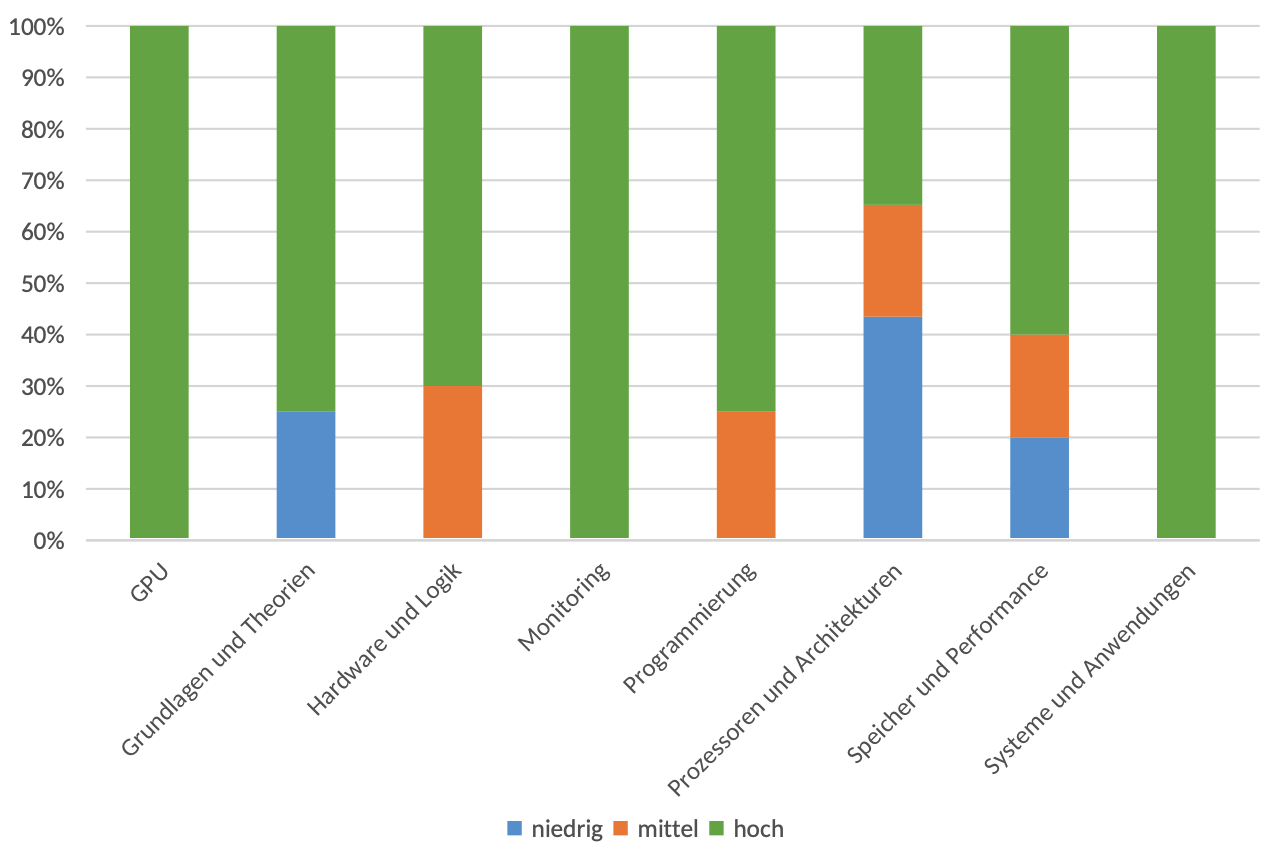
\includegraphics[width=0.90\textwidth]{graphics_sim/16-bekanntheit-thema.png}
        \caption{Verteilung Bekanntheit auf Themen}
        \label{fig:16-bekanntheit-thema}
    \end{subfigure}
    %
    \caption{Analysen zur Bekanntheit}
    \label{fig:bekanntheit-gesamt}
\end{figure}

\TODO{Weiter ausführen zur Bekanntheit}
